\documentclass[a4paper,10pt]{scrartcl}
\usepackage[ngerman]{babel}
\usepackage[T1]{fontenc}
\usepackage[utf8]{inputenc}
\usepackage{float}
\usepackage{graphicx}
\usepackage{amsmath}
\usepackage{upgreek}
\usepackage{amssymb}
\usepackage{amsfonts}
\usepackage{amssymb}
\usepackage{lmodern}
\title{Statistik 2018}
\author{Benjamin Altmiks}
\date{2. Oktober 2018 - \today}
\begin{document}
\maketitle
\tableofcontents
\newpage
\section{Einführung}
\begin{quote}
    „ There are three kinds of lies: lies, damned lies and statistics.“ \newline Leonard Henry Courteney
\end{quote}
\subsection{Allgemein}
Die Statistik ist aufgeteilt in die Zusammenstellung von Zahlen und die statistische Methodenlehre. Die statistische Methodenlehre beeinhaltet die Desprektive (Durchschnittliche Berechnung) und Induktive (Schätzung und Testen) Statistik sowie die Wahrscheinlichkeitstheorie.
\subsection{Merkmale}
Merkmale können als \textbf{qualitativ – quantitativ} und \newline \textbf{diskret (Abzählbar) – stetig (Nicht Abzählbar)} definiert werden. \newline
Die Grundgesamtheit ist die Menge aller relevanten Merkmalsträger
\subsection{Skalenniveaus}
Man unterscheidet Skalenniveaus zwischen: \newline\newline
\textsc{Nominalskala}: Daten die in keine logische Reihenfolge gebracht werden können wie Farben oder das Geschlecht
\newline\newline\textsc{Odinalskala}: Können in logische Reihenfolge gebracht werden, aber nicht quantifiziert werden, das heißt man kann nicht mit ihnen rechnen. Ein Beispiel hierfür sind Schulnoten
\newline\newline\textsc{Kardinalskala}: Sind Daten die in logische Reihenfolge gebarcht werden können, sowie eine Differenzbildung sinnvoll und möglich.
\subsection{Skalendegression und Skalenprogression}
Ist eine Skalierung um Informationen angemessen und möglichst genau darzustellen.\newline
\textbf{Skalendegression}: Durch Informationsverlust können alle Merkmale nominal Skaliert werden, metrische Merkmale auch ordinal skaliert. Nur metrische Merkmale dürfen metrisch skalliert werden.\newline
\textbf{Skalenprogression}: Interpretation von mehr Informationen aus Merkmalen, als inhaltlich vertretbar. (Fehlinterpretation möglich) 
\newpage
\section{R-Studio-Grundlagen}
\subsection{Allgemeine Befehle}
Die wichtigsten Befehle in R und R-Studio sind:
\begin{table}[H]
    \begin{tabular}{|c|l|}\hline
Eingabe&Funktion\\\hline
?Befehl&Erklärung/Definition\\\hline
x = y bzw x <- y&Zuweisungsoperator\\\hline
ls()&Objektauflistung\\\hline
rm(x)&Objektlöschung(x)\\\hline
    \end{tabular}
    \label{tab:my_label}
\end{table}
\subsection{Mathematik}
\subsubsection{Taschenrechner}
Man kann R it R-Studio ganz einfach als Taschenrechner mit den richtigen Befehlen verwenden. Diese sind zum Beispiel: \newline
\begin{itemize}
    \item Addition, Subtraktion, Multiplikation und Division mit Zeichen (+,-,*,/)
    \item Exponentialoperationen $x^y$ , Logarithmus log(x) oder Wurzel sqrt(x) 
    
\end{itemize}
\subsubsection{Vektoren}
Vektoren sind eine Urliste von Daten eines Merkmals. Es kann sich dabei um ein nominales (String) oder ein Metrisches (int) Merkmal handeln, wobei das Nominale Merkmal immer das stärkere ist.
\begin{table}[H]
    \begin{tabular}{|l|l|}
    \hline
c(x,y,z) & Erstellen eines neuen Vektors\\\hline
x:y & Aufernanderfolgende Ganze Zahlen von x bis y\\\hline
seq(from = x, to = y, by = z) & Folgen variabler Folgen mit bestimmtem Abstand\\\hline
rep(c(x,y),z) & Wiederholen einer Folge x,y in neuem Vektor z mal\\\hline
    \end{tabular}
    \label{tab:my_label}
\end{table}
\newpage
Auch auf Vektoren können Rechneroperationen ausgeführt werden. Sollte ein Vektor kleiner als der andere sein, so wird dieser solange von vorne wiederholt, bis die Länge der beiden Vektoren gleich ist. Das selbe gilt für Vergleichsoperatoren:
\begin{table}[h]
    \begin{tabular}{|l|l|}\hline
sum(x) & Berechnet die Summe aller Elemente aus dem Vektor\\\hline
length(x) & Berechnet die Anzahl der Elemente im Vektor\\\hline
 < , > , = & Vergleichoperatoren\\\hline
 \& , | & Verknüpfung zwischen Vergleichen\\\hline 
\end{tabular}
\label{tab:my_label}
\end{table}
\subsubsection{Fuktionen}
In R können Funktionen einer reellen Variable definiert werden. Die Funktionen können mit Konstanten sowie Variablen Skalen bzw. Vektoren aufgerufen werden:
\begin{table}[h]
    \centering
    \begin{tabular}{|l|l|}\hline
f = function(x) {x+1} &  Erstellt eine Funktion x+1 \\\hline
f(y) & Aufrufen der Funktion mit Wert y\\\hline
data.frame(x,f(x)) & X als Vektor ergibt Wertetabelle\\\hline
print(data.frame(x,f(x)),row.names = FALSE) & Zeilennummer unterdrücken\\\hline
    \end{tabular}
    \label{tab:my_label}
\end{table}
\subsubsection{Graphen von Funktionen}
In R-Studio ist es außerdem möglich die bereits genannten Funktionen mithilfe von curve(f) zeichnen zu lassen. curve() hat einige nützliche Parameter:
\begin{itemize}
    \item from, to für den Definitionsbereich,
    \item add für die Überlagerung mehrerer Kurven,
    \item col für die Farbe der Kurve
    \item xlab, ylab, main für die Beschriftung der Abszisse, Ordinate, der Überschrift
    \item lwd für die Strichdicke der Kurve
\end{itemize}
Mit grid() kann man ein Gitter in den Graphen einzeichnen.
\subsubsection{Merkmale}
\begin{table}[h]
    \begin{tabular}{|l|l|}\hline
str()&Allgemeine Merkmalabfrage/Skalenniveau /\\\hline
is.numeric()&Metrische Merkmalabfrage\\\hline
is.ordered&Ordinale Merkmalabfrage\\\hline
is.factor&Nominae Merkmalabfrage\\\hline
as.numeric()&Umwandlung von Zeichenkette zu numerisch\\\hline
as.factor&Umwandlung in nominale Merkmale\\\hline
\end{tabular}
    \label{tab:my_label}
\end{table}
\subsection{Datenverarbeitung}
\subsubsection{Data Frames}
Urlisten mit mehreren Merkmalen können über eine Tabelle abgebildet werden\newline
\begin{itemize}
\item\textbf{data.frame(Vektor, Vektor,...)}: Zeilen = Objekte, Spalten = Merkmalen
\item Einzelne Objekte können durch Index \textbf{dataFrame[x,y]} ausgegeben werden (Matrix)
\item Einzelne Spalten können durch Namen direkt angesprochen werden:\newline \textbf{dataFarame\$Namen}
\item Bedingungen für Spaltenabfrage durch \textbf{dataFrame[bedingung]} mit ursprünglichem Namen!
\item \textbf{nrow()} und \textbf{ncol()} gibt die Anzahl der Reihen/Zeilen aus
\item \textbf{rbind()} und \textbf{cbind()} kann die Tabelle um Objekte/Merkmale erweitern 
\end{itemize}

\subsubsection{Daten einlesen}
Zum einlesen von Daten kann in der Benutzeroberfläche von R-Studio mit $"$Import Dataset$"$ eine URL oder eine lokale Datei verwendet werden. Alternativ kann der Befehl $"$read.csv()$"$ verwendet werden.
Zur Verwendung dieser Datensätze kann ein Überblick geschaffen werden mit:
\begin{itemize}
    \item str(): Darstellung der Struktur
    \item head(): Ersten Objekte werden angezeigt
    \item summary(): Verteilung der Ausprägungen
\end{itemize}
\newpage
\section{Deskriptive Statistik}
\subsection{Notationen}
Es gelten im allgemeinen folgende Notationen:
\begin{itemize}
    \item X: Merkmalsvariable
    \item x: Realisation einer Merkmalsvariable
    \item i: Index, indiziert die Merkmalsträger (i = 1,....,n)
    \item n: Anzahl der Merkmalsträger
    \item \(a_j\): Merkmalsausprägung, also alle Merkmale ohne Duplikate
    \item h(\(a_j\)): Absolute Häufigkeit des Auftretens (H(\(a_j\)) für kumulativ = anhäufend)
    \item f(\(a_j\)): Relative Häufigkeit = Absolute Häufigkeit/n (F(\(a_j\)) für kumulativ)
\end{itemize}
Des weiteren gibt es die Urliste. Sie stellt das direkte Ergebnis einer Datenerhebung (Vektor der Merkmalsausprägungen) dar. Sie kann unsortiert oder sortiert vorliegen.
\subsection{Empirische Verteilungsfunktion}
Sei X eine Zufallsgröße mit der Verteilungsfunktion F und sei (x1, x2, …, xn) eine konkrete Stichprobe von X vom Umfang n. Unter der empirischen Verteilungsfunktion dieser Stichprobe versteht man die Funktion
\begin{eqnarray*}{F}_{n}(x)=\frac{{H}_{n}(x)}{n},\,\,x\in {\mathbb{R}},\end{eqnarray*}
In R-Studio berechenbar durch ecdf(x)
\subsection{(Empirische) Quantile}
Unter dem (unteren) empirischen p-Quantil Qp, (0 < p < 1) versteht man die Größe, die die geordnete Stichprobe so zerlegt, daß p * 100\% der n Daten kleiner als Qp sind. Sie ist exakt wie folgt definiert:
\begin{eqnarray*}K(x):=\left\{\begin{array}{ll}\displaystyle \sum _{i=-\infty }^{\infty }{(-1)}^{i}{e}^{-2{i}^{2}{x}^{2}} & {\text{f}\rmfamily{\ddot{u}}\text{r}}\,x\gt 0\\ 0 & {\text{f}\rmfamily{\ddot{u}}\text{r}}\,x\le 0\end{array}\right.\end{eqnarray*}
In R-Studio berechenbar durch quantile(x)
Zur Berechnung der Quantile ist mit folgendem Verfahren zu arbeiten:
\begin{enumerate}
    \item Es wird die eine sortierte Liste der Werte benötigt (aufsteigend)
    \item Wir berechnen n*p (n = Anzahl Werte, p = Quantil)
    \item Formel auswählen und Werte heraussuchen:
    \begin{align*}\tilde{x}_p=\begin{cases} \frac{1}{2}(x_{np}+x_{np+1}) & \text{ wenn }np\text{ ganzzahlig}\\ x_{\lceil np \rceil}& \text{ wenn }np\text{ nicht ganzzahlig}\end{cases}
\end{align*}

\end{enumerate}
\subsection{Lageparameter}
\subsubsection{Modus}
der Modus ist der häufigste Wert, der in der Stichprobe vorkommt. Es kann auch mehrere Modi geben, wenn zwei oder mehrere verschiedene Merkmale gleich oft am häufigsten vorkommen. Er ist Sinnvoll bei allen Skalenniveau
\subsubsection{Median}
Ist X eine auf dem Wahrscheinlichkeitsraum $({\rm{\Omega }},{\mathfrak{A}},P)$ definierte reelle Zufallsvariable, so wird jede Zahl m mit der Eigenschaft $P(X\le m)\ge \frac{1}{2}\quad \text{und}\quad P(X\ge m)\ge \frac{1}{2}$
als Median der Verteilung von X bzw. als Median von X bezeichnet. Es ist der Mittlere Wert in einer sortierten Liste und wird in R durch median(x) berechnet.
\subsubsection{Arithmetisches Mittel/Durchschnitt}
Arithmetisches Mittel aus n Beobachtungen (x1, x2, …, xn) einer Zufallsgröße X, also 
\begin{eqnarray*}\overline{x}:=\frac{1}{n}\displaystyle \sum _{i=1}^{n}{x}_{i}.\end{eqnarray*}
In R-Studio berechenbar durch mean(x)
\newpage
\section{Streuungsparameter}
\subsection{Graphische Darstellungen in R}
In R können Daten wir folgt dargestellt werden:
\begin{itemize}
    \item Durch R bestimmtes passende Graphische Darstellung: plot(Data\$SubData)
    \item Balkendiagramm:barplot(Daten)
    \item Säulendiagramm:barplot(Daten, horiz = T)
    \item Kreissektorendiagramm:pie(Daten)
    \item Farben: plot(Daten ,col = c("blue"...))
    \item Histogramm (für klassierte Daten): truehist(Daten)
    \item Dichteplot: polygon(Daten,density, col)
    \item Gegenüberstellung:
    \begin{itemize}
        \item Zwei metrische Merkmale (Streuplot), 
        \item Zwei nominale Merkmale (Spinplot), 
        \item Einem metrisches und einem nominales Merkmal (Boxplot)
        \item Mehrere metrische Merkmale (Streuplotmatrix)
    \end{itemize}
\end{itemize}
barplot(häufigkeitstabelle) = Balkendiagramm bzw Säulendiagramm --> horiz kann drehen
pie(häufigkeitstabelle) = kreisdiagramm
\begin{itemize}
    \item Spannweite:\begin{eqnarray*}R={x}_{max}-{x}_{min},\end{eqnarray*}
    \item Mittlere Quadratische Abweichung (Qualitätskriterium für Schätzer)
    \begin{eqnarray*}{s}^{2}=\frac{1}{n}\displaystyle \sum_{i=1}^{n}{({x}_{i}-\overline{x})}^{2}\end{eqnarray*}
    \item Empirische Standardabweichung 
    \begin{eqnarray*}
    S = \sqrt{{s}^{2}}
    \end{eqnarray*}
    \item Variationskoeffizient 
    \begin{eqnarray*}\upsilon =\frac{s}{x}.\end{eqnarray*}
\end{itemize}
\newpage
\subsection{Boxplot}
Graphisch kann dies mithilfe eines Boxplots gezeigt werden. Ein Box-Whisker-Plot ist eine Zusammenfassung eines Datensatzes in fünf Punkten. Diese fünf Punkte sind das Minimum, das untere Quartil, der Median, das obere Quartil und das Maximum.\newline
Das Minimum und Maximum (Whisker) sind beschränkt durch das 1.5 Fache des Quartilsabstandes. Alle darüber hinausliegenden Werte werden als Ausreißer bezeichnet und extra mit einem Kreis makiert.
\begin{figure}[h] 
  \centering
      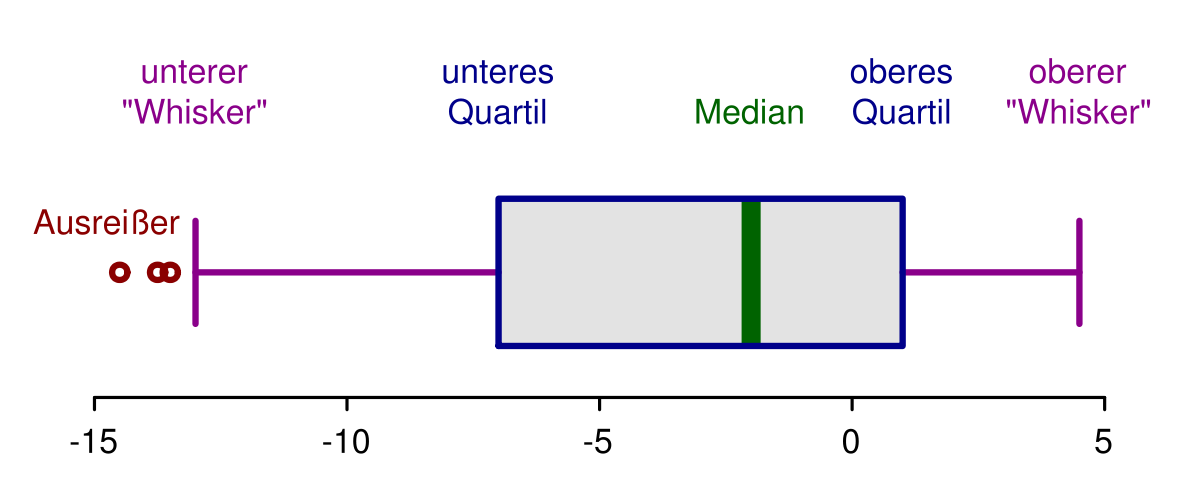
\includegraphics[width=0.9\textwidth]{Boxplot.png}
  \label{fig:Bild1}
\end{figure}
\section{Konzentrationsmaße}
Konzentrationsmaße messen, wie ungleich bzw. wie geballt konzentriert Messwerte der Merkmalsträger verteilt sind (relative Konzentrationsmaße). Mithilfe einer Lorenzkurve kann der Gini Koeffizient berechnet werden.
\subsection{Lorenzkurve}
Die Lorenzkurve ist eine graphische Darstellung der Verteilung.
Zum zeichnen einer Lorenzkurve geht man wie folgt vor:
\begin{enumerate}
    \item In einer sortierten Liste berechnet man zunächächt den kumulierten \textbf{Anteil an der Grundmenge} und erhält dadurch die x-Koordinaten:
    \begin{align*}
    u_k&=\frac{j}{n}
    \end{align*}
    \item Für die y-Koordinaten wird der kumulierte Anteil an der Merkmalssumme berechnet, wobei die Merkmalssumme berechnet wird durch:
    \begin{align*}
    Q=\sum_{i=1}^n x_i
    \end{align*}
    Die eigentliche Koordinate ergbit dich dann durch die Berechnung:
    \begin{align*}
    v_j=\frac{\sum_{i=1}^j x_i}{Q}
    \end{align*}
\end{enumerate}

\subsection{GiniKoeffizient-TODO}
\section{Streuungsdiagramm}
Ein Streuungsdiagramm wird verwendet wenn in einer Stichprobe viele verschiedene Ausprägungen bze. Merkmale vorhanden sind. Es werden dabei alle Merkmale mit einem Punkt in ein kartesisches Koordinatensystem eingetragen, wodurch sich eine Punktwolke ergibt. Man erhofft sich durch das Muster der Punkte im Streudiagramm Informationen über die Abhängigkeitsstruktur der beiden Merkmale zu erkennen, die durch die Koordinaten repräsentiert sind.
TODO
\newpage
\section{Zweidimensionale Urliste}
\subsection{Kontingenztabelle}
Über Kontingenztabellen können zwei Merkmale X und Y, z. B. ein ordinal- mit einem nominalskalierten, in Beziehung gebracht werden, um die Zusammenhänge der Merkmalsausprägungen strukturiert als Häufigkeiten h (siehe Klassenbildung) darstellen zu können. Des weiteren können folgende Häufigkeiten in einer Kontingenztabelle dargestellt werden:
\begin{figure}[h] 
  \centering
    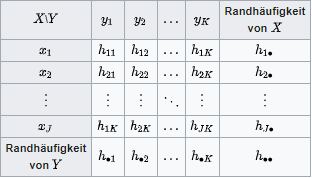
\includegraphics[width=0.9\textwidth]{Kontingenztabelle.PNG}
  \label{fig:Bild1}
\end{figure}
\begin{itemize}
    \item Gemeinsame Häufigekit: Die Elemente in der Tabelle, die darstellen welche Stichproben auf beide Bedingungen zutreffen
    \item Absolute Randhäufigkeit: Summer alle absoluten Häufigkeiten in dieser Spalte/Zeile
    \item Bedingte (relative) Häufigkeit: Summer alle relativen Häufigkeiten in dieser Spalte/Zeile
\end{itemize}
$\Rightarrow$ Hierdurch kann einfach ein allgemeines Bild von Ursache und Wirkung erstellt werden.
\subsection{Korrelationskoeffizient}
Der Korrelationskoeffizient ist ein Maß für die Abhängigkeit (Assoziation) zwischen Zufallsgrößen. Man nennt X und Y positiv bzw. negativ korreliert, falls $\varrho$xy > 0 bzw. $\varrho$xy < 0 gilt. Ist $\varrho$xy = 0, d. h. cov(X, Y) = 0, so heißen X und Y unkorreliert. Aus der stochastischen Unabhängigkeit zweier Zufallsgrößen folgt ihre Unkorreliertheit.
\begin{eqnarray}{\varrho }_{xy}=\frac{cov(X,Y)}{{\sigma }_{x}{\sigma }_{y}}\end{eqnarray} wobei gilt:
\begin{eqnarray}-1\le {\varrho}_{xy}\le +1\end{eqnarray}
\subsection{Multipler Korrelationskoeffizient}
Als multiplen Korrelationskoeffizienten $\varrho$1(2···m) zwischen X1 und (X2, …, Xm) bezeichnet man den einfachen Korrelationskoeffizienten zwischen X1 und gX1 (X(2)), X(2) = (X2, …, Xm) d. h., es ist ein Maß für die lineare Abhängigkeit zwischen X1 und der Gesamtheit der X2, …, Xm
\begin{eqnarray}{\varrho }_{1(\mathrm{2\cdots}m)}=\frac{{cov}({X}_{1},{g}_{{X}_{1}}({X}^{(2)})}{\sqrt{Var({X}_{1})Var({g}_{{X}_{1}}({X}^{(2)}))}}.\end{eqnarray}
\newpage
\section{Lineares Modell}
Ein lineares Modell wird verwendet, um einen bestimmten Erwartungswert Y\footnote{Regressand bzw. abhängige Variable} durch eine bestimmten lineare mit X\footnote{Regressor bzw. unabhängige Variable} Weise zu berechnen, die von einer gewissen Bedingungskonstellationen abhängt. Allgemein gilt:
\begin{eqnarray*}
y = f(x)
\end{eqnarray*}
Für einfache lineare Schätzungen (auch lineare Regression genannt) gilt:
\begin{eqnarray*}
yi = a + bxi + \epsilon i
\end{eqnarray*}
$\epsilon$: Fehler der Grundgesamtheit
\subsection{Residuum}
Abweichung zwischen gegebenen Daten der Stichprobe und durch Modell geschätzten Werten
\begin{eqnarray*}Q(a,b)=\mathop{\sum ^{\infty }}\limits_{n=-\infty }{a}_{n}{(z-{z}_{0})}^{n},\end{eqnarray*}
(\={x}; \={y}) ist Datenschwerpunkt und liegt \textbf{immer} auf der Regrassionsgeraden!
\subsection{Fehlerquadratsumme}
TODO
\subsection{Varianz und Information}
Die Varianz ist ein Maß für die Streuung der Wahrscheinlichkeitsdichte um ihren Schwerpunkt. Sie wird definiert als die mittlere quadratische Abweichung einer reellen Zufallsvariablen von ihrem Erwartungswert.
\subsection{Determinationskoeffizient}
Der Determinationskoeffizient ist ein Maß für die Abweichungen der Vorhersagen eines Regressionsmodells von den empirischen Daten, also ein Maß für die Modellanpassung. Konkret entspricht dies dem Anteil der Variation der Modellvorhersagen, der sogenannten erklärten Summe der Abweichungsquadrate, an der Variation der beobachteten Werte der abhängigen Variablen, der sogenannten Gesamtsumme der Abweichungsquadrate. Er wird interpretiert als der durch die Regression erklärter Anteil der Varianz.
\newpage
\section{Kombinatorik}
Die Kombinatorik ist ein Teilgebiet der Mathematik, in dem man die Eigenschaften und die Struktur der Abbildungen (oder Morphismen) einer endlichen Menge in eine Menge von Objekten, welche gewisse Bedingungen erfüllen, studiert. Die Kombinatorik beschäftigt sich vor allem mit dem Zählen und Ordnen der Morphismen.
\subsection{Permutation}
Die Permutation ist die "Anordnung von n Objekten". Für n unterschiedliche Objekte kann man n! verschiedene Anordnungen vornehmen.\newline
Für n Objekte in k Gruppen mit jeweils
$n_k (n_1,n_2,n_3...,n_k)$ 
nicht unterscheidbaren Elementen können in
\begin{eqnarray*}
\frac{n!}{n_1!*n_2!*...*n_k!}
\end{eqnarray*}
verschiedenen Varianten angeordnet werden.
\subsection{Auswahl von k-Objekten aus n-Elementen}
\begin{tabular}{|l|c|c|} \hline
 & mit Wiederholung & ohne Wiederholung \\\hline
mit Reihenfolge & n$^{k}$ & $\frac{n!}{(n-k)!}$ \\\hline
ohne Reihenfolge & $\binom{n+k-1}{k}$ & $\binom{n}{k}$  \\\hline
\end{tabular}\\
Hilfe für Berechnung mit Taschenrechner siehe Kapitel Taschenrechner
\section{Zufall und Wahrscheinlichkeit}
\begin{itemize}
    \item Zufallsvorgang: Geschechen mit ungewissem Ausgang (z.B Münzwurf)
    \item Elementarereignis $\omega$: Ein möglicher Ausgang (Kopf). Elementarereignis schließt sich gegenseitig aus.
    \item Ergebnismenge $\Omega$: Menge aller $\omega$
    \item Ereignis A: Folgeerscheinung eines Elemantarereignisses. Ereignisse schließen sich nicht gegenseitig aus
    \item Wahrscheinlicheit P(A): Chancen für das Eintreten von A
    \item Laplace-Wahrscheinlichkeit:
    \begin{align*}
    P(A) = \frac{A}{\Omega} = 
    \frac{\text{Anzahl der für A günstigen Fälle}}{\text{Anzahl aller möglichen Fälle}}
    \end{align*}
\end{itemize}
\subsection{Laplace Wahrscheinlichkeit und das Urnenmodell}
In einem Urnenmodell werden n Objekte aus einer Menge mit N Objekten gezogen. Dabei gilt:
\begin{itemize}
    \item Ziehen mit Zurücklegen : $N^n$
    \item Ziehen ohne Zurücklegen : $\frac{N!}{N-n}$
\end{itemize}
Dabei gelten folgende Rechenregeln:
\begin{enumerate}
    \item P(A) a$\leq$b
    \item A $\subseteq$ B $\Rightarrow$ P(A)$\leq$P(B)
    \item P(A$\cup$B) = P(A) + P(B) - P(A$\cap$B)
\end{enumerate}
\subsection{Bedingte Wahrscheinlichkeit}
Eine Bedingte Wahrscheinlichkeit beschreibt ein Ereignis, das sich verändert, wenn bereits ein anderes Ereigniss eingetreten ist. Dabei ist $P_B(A)$ bzw P(A|B) die Wahrscheinlichleit von A unter der Bedingung, dass B eingetreten ist. Es gilt:
\begin{eqnarray}
P_B(A) = \frac{P(A \cap B)}{P(B)}
\end{eqnarray}
Also, das die Wahrscheinlichkeit von A unter der Bedingung B [$P_B(A)$] gleich dem Quotienten der Wahrscheinlichkeit von A und B [P(A$\cup$B)] und der Wahrscheinlichkeit von B ist. [P(B)]
\section[Zufallsvariablen und Verteilungen]{Zufallsvariablen und Verteilungen\footnote{Skript Seite 144}}
\subsection{Zufallsvariablen}
Eine Funktion X, die jedem Ergebnis $\omega$ des Ergebnisraum $\Omega$ genau eine Zahl x der Menge der reellen Zahlen $\mathbb{R}$
zuordnet (disjunkt), heißt Zufallsvariable, bzw:
\begin{eqnarray*}
X: \Omega \rightarrow \mathbb{R}
\end{eqnarray*}
Notationen am Beispiel des 2-fachen Würfelwurfs mit y als Augensumme:
\begin{itemize}
    \item $\Omega$ = {(1,1); (1,2); ...; (6,6)} = Menge aller Elemente
    \item $y(\Omega)$ = {2, 3, 4, ..., 12} = Endlicher Wertebereich
    \item P(Y$\leq$4) = $\frac{6}{36}$ = P(Y<5)
    \item P(3$\leq$X$\geq$5) = 
\end{itemize}
\subsection{Diskrete Zufallsvariablen}
Eine Zufallsvariable X heißt diskret, wenn die Ergenbismenge endlich ist. Diskrete Zufallsvariablen entstehen meist durch einen Zählvorgang.\\
Eine Wahrscheinlichkeitsverteilung/verteilungsfunktion gibt an, wie sich die Wahrscheinlichkeiten auf die möglichen Werte einer Zufallsvariablen verteilen.
\begin{figure}[h] 
  \centering
    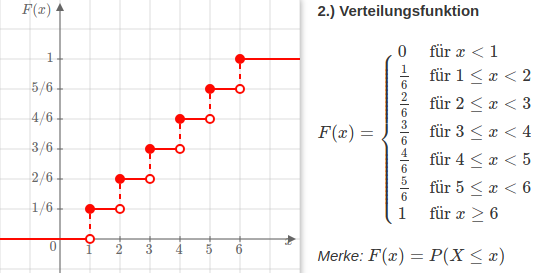
\includegraphics[width=0.9\textwidth]{Verteilungsfunktion.png}
  \label{fig:Bild1}
\end{figure}

\subsubsection{Binomialverteilung B(n, p)}
Die Binomialverteilung ist eine von den Parametern n $\in$ $\mathbb{N}$ und p $\in [0,1]$ abhängende diskrete Wahrscheinlichkeitsverteilung. Dabei ist n = Anzahl der Durchführungen (jeweils unabhängig) und p = P(A) = Wahrscheinlichkeit für A. Es gilt:
\begin{eqnarray*}
\binom{n}{k} * p^k * (1-p)^{n-k}
\end{eqnarray*}
\subsubsection[Hypergeometrische Verteilung Hyp(N, M, n)]{Hypergeometrische Verteilung Hyp(N, M, n)\footnote{Skript Seite 153}}
Die Hypergeometrische Verteilung ist eine Wahrscheinlichkeitsverteilung für ein n-faches Ziehen. Im Gegensatz zur Binomialwahrscheinlichkeit wird ein ziehen \textbf{ohne} Zurücklegen aus N Objekten durchgeführt, wobei M markiert sind.
\begin{quote}
X = Anzah gezogener Objekte mit Markierung
\end{quote}
$\Rightarrow$ Hypergeometrisch Verteilt mit Parametern N, M, n bzw. $X \sim Hyp(N;M;n)$\\
Allgemein gilt:
\begin{eqnarray*}
{h}_{N,M,n}:\{0,\ldots, n\}\ni m\to \frac{\left(\begin{array}{c}M\\ n\end{array}\right)\left(\begin{array}{c}N-M\\ n-m\end{array}\right)}{\left(\begin{array}{c}N\\ n\end{array}\right)}\in [0,1]
\end{eqnarray*}
Wie zu erkennen wird angegeben wie viele Treffer und wie viele Nichttreffer es geben soll. Dies wird durch die Gesamtanzahl des Biomialkoeffizienten geteilt. In R:
\begin{itemize}
    \item dhyper(x = 2, m = 6, n = 43,  k = 6, lower.tail = FALSE) = 0.132378\\
    $\Rightarrow$ Genau 2 (von 6) aus (insgesamt) N = 49 (n = N-m)
    \item phyper(q = 2, m = 6, n = 43,  k = 6, lower.tail = FALSE) = 0.9813625\\
    $\Rightarrow$ Höchstens 2 (von 6) aus (insgesamt) 49
\end{itemize}
\subsubsection[Poissonverteilung]{Poissonverteilung P($\lambda$)\footnote{Skript Seite 156}}
Die Poissonverteilung\footnote{Eine Herleitung zum Verständnis ist nicht gegeben/gefordert } ist eine Wahrscheinlichkeitsverteilung, mit der die Anzahl von Ereignissen modelliert werden kann, die bei konstanter mittlerer Rate unabhängig voneinander in einem festen Zeitintervall eintreten.
\begin{quote}
    X = 'Anzahl der <Ereignisse> pro <Zeitintervall>' mit $X \sim P(\lambda)$
\end{quote}
Für die Zufallsgröße X (poissonverteilt mit Parameter $\lambda$)gilt:
\begin{align*}
\mathbb{P}(X=k)&=\frac{\lambda^k}{k!}e^{-\lambda}
\end{align*}
Ein Berechnung kann des weiteren über die Tabelle der Poissonverteilung bestimmt werden.
In R:\\
$\Rightarrow$ dpois(x = 2, lambda = 0.0998) = 0.00450701
\subsection[Stetige Zufallsvariablen]{Stetige Zufallsvariablen \footnote{Skript Seite}}

\subsubsection{Stetige Gleichverteilung}
Eine Zufallsvariable X wird als stetig bezeichnet, wenn sie überabzählbar unendlich viele Werte annimmt.
Eine Wahrscheinlichkeitsverteilung gibt an, wie sich die Wahrscheinlichkeiten auf die möglichen Werte einer Zufallsvariablen verteilen.
\subsubsection{Dichtefunktion}
Die Dichtefunktion ist ein Hilfsmittel zur Beschreibung einer stetigen Wahrscheinlichkeitsverteilung. Dabei ist der Flächeninhalt zwischen der Dichtefunktion und der X-Achse gleich die Wahrscheinlichkeit der stetigen Zufallsvariable X.
Es gilt:
\begin{equation*}
F(x) = P(X \le x) = \int_{-\infty}^{x} \! f(u) \, \mathrm{d}u    
\end{equation*}
Dabei muss gelten:
\begin{itemize}
    \item $f(x) \geq 0$ $\Rightarrow$ Dichtefunktion kann nur positive Werte annehmen 
    \item $\int_{-\infty}^{\infty} \! f(x) \, \mathrm{d}x = 1$ $\Rightarrow$ Die Fläche unter der Dichtefunktion hat den Inhalt 1
\end{itemize}
In R:
\begin{itemize}
    \item dunif(Vektor, min = a, max = b) $\Rightarrow$ Verteilungsfunktionn
    \item punif(Vektor, min = a, max = b) $\Rightarrow$ Quantilsfunktion
\end{itemize}
\subsubsection{Verteilungsfunktion}
Eine Funktion F, die jedem x einer Zufallsvariablen X genau eine Wahrscheinlichkeit $P(X \le x)$ zuordnet, heißt \textbf{Verteilungsfunktion}.\\
Es gilt Allgemein: $F: x \rightarrow P(X \le x)$

\subsubsection{Gleichverteilung}
Wie bei der diskreten Gleichverteilung ist auch bei der stetigen Gleichverteilung jedes Ergebnis gleich wahrscheinlich. Der Unterschied ist, dass wir diesmal alle Werte aus einem Intervall [a,b] betrachten (statt einzelner Werte bei der diskreten Gleichverteilung). Manchmal spricht man auch von der Rechteckverteilung. Es gilt also:
\begin{eqnarray*}
f:{\mathbb{R}}\ni x\to \left\{\begin{array}{rl}\frac{1}{b-a}, & a\lt x\lt b\\ 0, & x\notin(a,b)\end{array}\in {\mathbb{R}}.\right.
\end{eqnarray*}

\begin{figure}[h] 
  \centering
      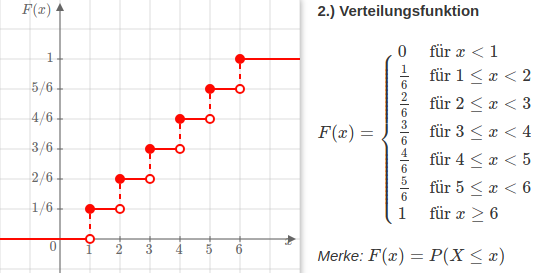
\includegraphics[width=0.9\textwidth]{Verteilungsfunktion.png}
  \label{fig:Bild1}
\end{figure}
\newpage
\subsubsection{Normalverteilung}
Der Parameter $\mu\in\mathbb{R}$ steht dabei für den Erwartungswert/Lageparameter und $\sigma^2>0$ für die Varianz (bzw. $\sigma$ für die Standardabweichung/Streuungsparameter) der Verteilung. Die Funktion/Glockenkurve ist dabei immer Symmetrisch um den Lagerparameter. (Symmetrisch zu $\mu$)
\begin{align*}
f(x)=\frac{1}{\sigma\sqrt{2\pi}}e^{-\frac{(x-\mu)^2}{2\sigma^2}}
\end{align*}
\textbf{Standartnormalverteilung:}
Für N(0,1) und F(x) = $\Phi$(x) $\Rightarrow$ Tabelle ablesbar\\
Allgemein gilt:
\begin{eqnarray}
1. F(x) = \Sigma(\frac{x-\mu}{\omega})
2. \Phi(-x) = 1-\Phi(x)
3. F(x) = 0.5 \Rightarrow x = \mu
4. F(x_1) = 1 - F(x_2) \Rightarrow \mu = \frac{x_1+x_2}{2}
\end{eqnarray}
In R gilt:
\begin{itemize}
    \item dnorm(x (Vektor Quantile), mean = 0 (Mittel), sd= 0 (Standartabweichung))
    $\Rightarrow$ Dichtefunktion
    \item pnorm(q (Vektor Quantile), mean = 0 (Mittel), sd= 0 (Standartabweichung)), 
    $\Rightarrow$ Verteilungsfunktion
    \item qnorm (Vektor Wahrscheinlichkeit, mean = 0 (Mittel), sd= 0 (Standartabweichung))
    $\Rightarrow$ Quantilfunktion
\end{itemize}
Für die Lineare Transformation gilt:
\begin{eqnarray}
\tilde{Y} = \frac{Y - \mu}{\sigma}
\end{eqnarray}
\subsubsection{Lagerprameter}
\begin{itemize}
    \item Modus: Häufigster Wert (Nicht allgemein Definiert)\\
    $\Rightarrow$ Normalverteilung: $x_mod = \mu$
    \item Median: Mittlerer Wert
    $\Rightarrow$ Normalverteilung: $x_mod = \mu$ 
    \item $\beta$-Fraktil bzw. $\beta$-Quantil: Flächeninhalt der (stetigen) Dichtefunktion
    $\Rightarrow$ Interpolation Berechnung: $\x_\beta \approx (x_b - x_a)*\frac{\beta - a}{b-a} X$
    \item Erwartungswert E(x) bzw $\mu$: Unterscheidung zwischen diskret und stetig:\\
    $\Rightarrow$ Diskret: E(x) = $\sum_{i=1}^{} x_i * f(x_i)$\\
    $\Rightarrow$ Stetig-Exponentialverteilt E(X): $\int _{-\infty }^{+\infty }x$ * f(x) dx
\end{itemize}
\subsubsection{Rechenregeln für den Erwartungswert}
\begin{itemize}
    \item Symmetrie von f bezüglich a: E(X) = a
    \item Lineare Transformation: E(a+bX) = a + b * E(X)
    \item Summenbildung: E($\sum_{i=1}^n X_i$) = $\sum_{i=1}^n E(X_i)$
    \item Unabhängigkeit: X, Y unabhängig $\Rightarrow$ E(X*Y) = E(X) * E(Y)
\end{itemize}
\subsubsection{Streungsparameter}
\begin{itemize}
    \item Varianz Var(X) bzw $\sigma^2$:
    $\Rightarrow$ 
    \item Standartabweichung $\sigma$: Sta(X) = \sqrt{Var(X)}
\end{itemize}

\subsubsection{Rechenregeln für die Varianz}
\begin{itemize}
    \item $Var(X) = E(X^2)- [E(X)]^2$
    $\Rightarrow$ 
\end{itemize}

% Ende 27.11 Seite 176
% Aufgaben bis 84




\section{Taschenrechner}
\begin{enumerate}
    \item Häufigkeiten einschalten:
    $\Rightarrow$ SHIFT + SETUP + DOWN + 3 (Statistik)
    \item Statistik-Modus
    $\Rightarrow$ MENU + 6 + 1 (Variable)
    \item Daten und Häufigkeiten eingeben
    $\Rightarrow$ Abschluss der Dateneingabe durch AC
    \item Ergebnisse/Maßzahlen
    \item OPTN + 2 (1-Variab-Bereich)
\end{enumerate}
Dabei kann folgendes abgelesen werden:
\begin{table}[]
    \begin{tabular}{|r|l|}\hline
    \end{tabular}
\end{table}
\subsection{zu 9.2}
\begin{tabular}{|l|c|c|} \hline
 & mit Wiederholung & ohne Wiederholung \\\hline
mit Reihenfolge & n$^{k}$ & Zahl+Shift+nPr(*)+Zahl \\\hline
ohne Reihenfolge & (Formel)+Shift+nCr(/)+Zahl &  Zahl+Shift+nCr(/)+Zahl \\\hline
\end{tabular}
\end{document}